\appendix
\appendixpage
\addappheadtotoc
%
% \begin{figure}%[H]
%   \begin{center}
%   \includegraphics[width=0.8\textwidth]{}
%   \end{center}
%   \caption{Left panel shows data over the quake location, right panel shows data over the ribbon location. From top to bottom, plots show lightcurves from IRIS Si IV, Mg II, Balmer wavelengths and Mg II wing, with the bottom panel showing the lightcurve from SDO HMI.}\label{lcseries-bold}
% \end{figure}

%insert figure showing ribbon coords oplot
%\graphicspath{ {~/PhD/Thesis/upgrade-plots/}}


%contains energy time plots for quake and ribbon locations
%also contains energy tables


%\includegraphics[trim=left bottom right top, clip]{file}
\section{Equations}\label{mhdeqns}
\paragraph{Maxwell's Equations and Ohm's Law}
Maxwell's equations and Ohm's law describe electromagnetism in terms of magnetic induction $\vec{B}$, magnetic permeability of free space $\mu$, electric field $\vec{E}$, electrical permittivity of free space $\epsilon_{0}$, charge density $\rho_{c}$ and electric current density $\vec{j}$ \\ 

\textbf{Ampère's Law}
\begin{equation}\label{max1:ampere}
\nabla\times\vec{B}=\mu_{0}(\vec{j}+\epsilon_{0}\frac{\partial \vec{E}}{\partial t})
\end{equation}

\textbf{Faraday's Law}
\begin{equation}\label{max2:faraday}
\nabla\times\vec{E}=-\frac{\partial \vec{B}}{\partial t}
\end{equation}

\textbf{Gauss's Law}
\begin{equation}\label{max3:gauss}
\nabla\cdot\vec{E}=\frac{\rho_{c}}{\epsilon_{0}}
\end{equation}

\textbf{No Magnetic Monopoles}
\begin{equation}\label{max4:nomonopole}
\nabla\cdot\vec{B}=0
\end{equation}

with Ohm's law as,

\begin{equation}\label{ohmslaw}
\vec{j}=\sigma(\vec{E}+\vec{v}\times\vec{B})
\end{equation}

where $\sigma$ is electrical conductivity. 

\paragraph{Fluid Dynamics Equations}
The fluid dynamics relations are written in terms of density $\rho$, velocity $\vec{v}$, time $t$, pressure $p$, gas constant $\Re$ and temperature $T$. 
%$\frac{d}{dt}=\frac{\partial}{\partial t}+ \vec{v}\cdot\nabla$, sometimes reffered to as the material derivative, is a way of stating the rate of change with respect to time of the  

\begin{equation}\label{motion}
\rho\frac{d\vec{v}}{dt}=-\nabla p
\end{equation}
 
\begin{equation}\label{masscontinuity}
\frac{d\rho}{dt}+\rho\nabla\cdot\vec{v}=0
\end{equation}

\begin{equation}\label{perfectgaslaw}
p=\Re\rho T
\end{equation}

Equation \ref{motion} is the eqn. of motion describing how the forces are exerted on the fluid are equal to the negative gradient of plasma pressure. Equation \ref{masscontinuity} is the eqn. of mass continuity (mass is conserved), whilst equation \ref{perfectgaslaw} is the perfect gas law relating plasma pressure, density and temperature. 

\paragraph{MHD Equations}
Another way to write the relationship between $\vec{B}$ and $\vec{v}$ is the equation of motion \ref{motion} modified by the Lorentz force.

\begin{equation}\label{motion1}
\rho\frac{d\vec{v}}{dt}=-\nabla p+\vec{j}\times\vec{B}
\end{equation}

The pressure gradient $-\nabla p$ describes the change from high to low plasma pressure. The Lorentz force, $\vec{j}\times\vec{B}$ acts perpendicularly to the magnetic field, therefore accelerated plasma in a direction parallel to the magnetic field is caused by other forces. If equation \ref{new1} is substituted into the Lorentz force,
\begin{equation}\label{lorentzsub1}
\vec{j}\times\vec{B} = (\nabla\times\frac{\vec{B}}{\mu})\times\vec{B}
\end{equation}


\begin{equation}\label{maghydstat}
\rho\frac{d\vec{v}}{dt}= -\nabla p + (\vec{B}\cdot\nabla)\frac{\vec{B}}{\mu}-\nabla(\frac{B^2}{2\mu}) 
\end{equation}

Because $-\nabla(\frac{B^2}{2\mu}$ is in the same form as $-\nabla p$ it can be said to be the \emph{magnetic pressure}, providing a force pointing from high to low magnetic pressure as $B^2$ changes with position.

\paragraph{Reduced MHD Equations}
Based on assumptions:
\begin{itemize}
\item $v<<v_{c}$, typical plasma velocities are much slower than the sound speed 
\item All the effects of radiation, viscosity, electric charge density and displacement currents are negligable 
\end{itemize}
It is possible to reduce Maxwell's equations into the following form:

\textbf{Ampère's Law}
\begin{equation}\label{max1:ampere}
\nabla\times\vec{B}=\mu_{0}\vec{j}
\end{equation}

\textbf{Faraday's Law}
\begin{equation}\label{max2:faraday}
\nabla\times\vec{E}=-\frac{\partial \vec{B}}{\partial t}
\end{equation}

\textbf{Gauss's Law}
\begin{equation}\label{max3:gauss}
\nabla\cdot\vec{E}=0
\end{equation}

\textbf{No Magnetic Monopoles}
\begin{equation}\label{max4:nomonopole}
\nabla\cdot\vec{B}=0
\end{equation}

\section{Figures}\label{figures}

\begin{figure}[H]
  \begin{center}
  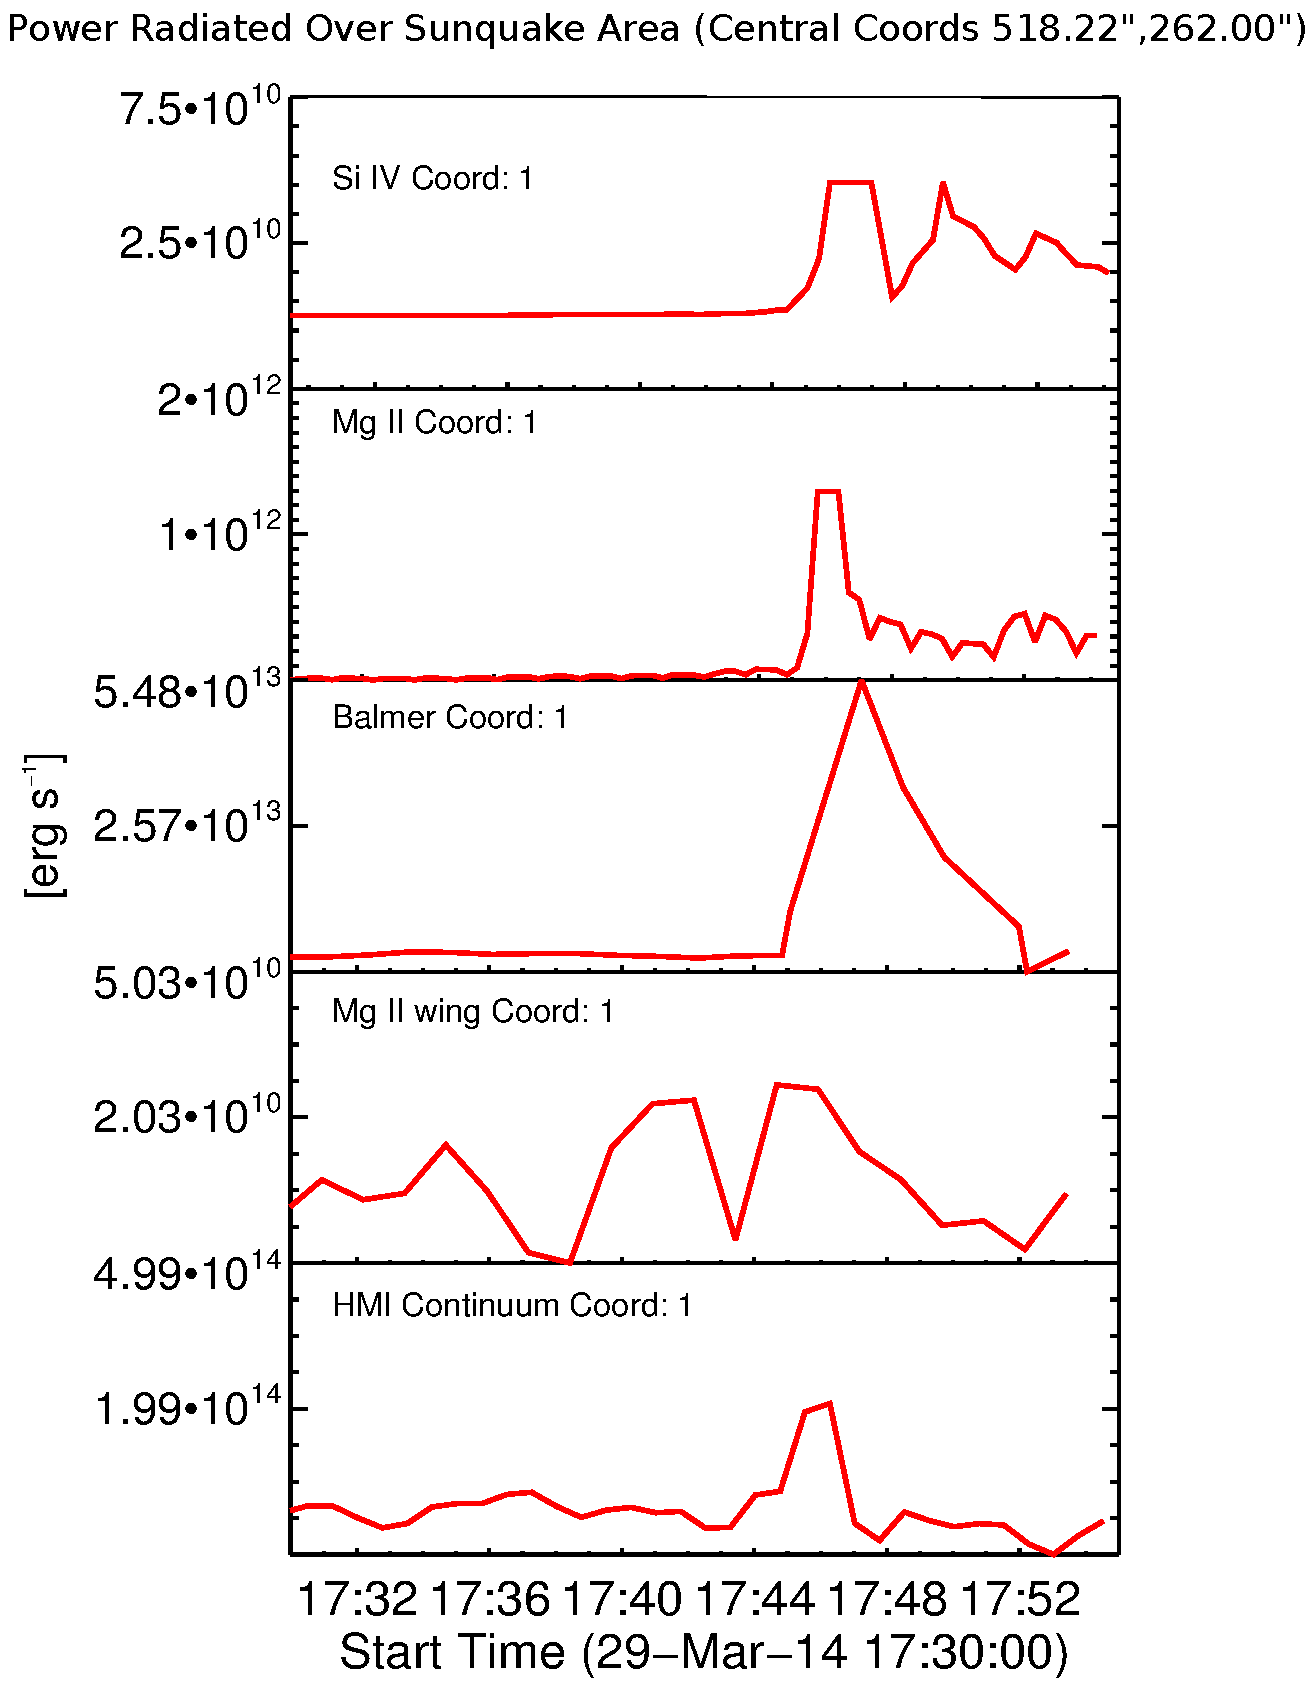
\includegraphics[width=0.6\textwidth]{29-Mar-14-Ribbon-Area-1-Sunquake-Area-Power-Ladder}
  \end{center}
  \caption{Shows radiative power from an area comparable to the sunquake impact, centered on region 1, relating to heliocentric coordinates 518.2", 262.0" which is directly over the sunquake location. Each plot represents an independant data set, in order from top to bottom the sets are; IRIS SJ 1400 \AA\ (Si IV); IRIS SJ 2796 \AA\ (Mg II); IRIS SG  2825.7 to 2825.8 \AA\ (Balmer Continuum); IRIS SJ 2832 \AA\ (Mg II wing); SDO HMI continuum (HMI).}\label{plot1}
\end{figure}
\begin{figure}[H]
  \begin{center}
  \textbf{Quake Location Energy Over Time}\par\medskip
  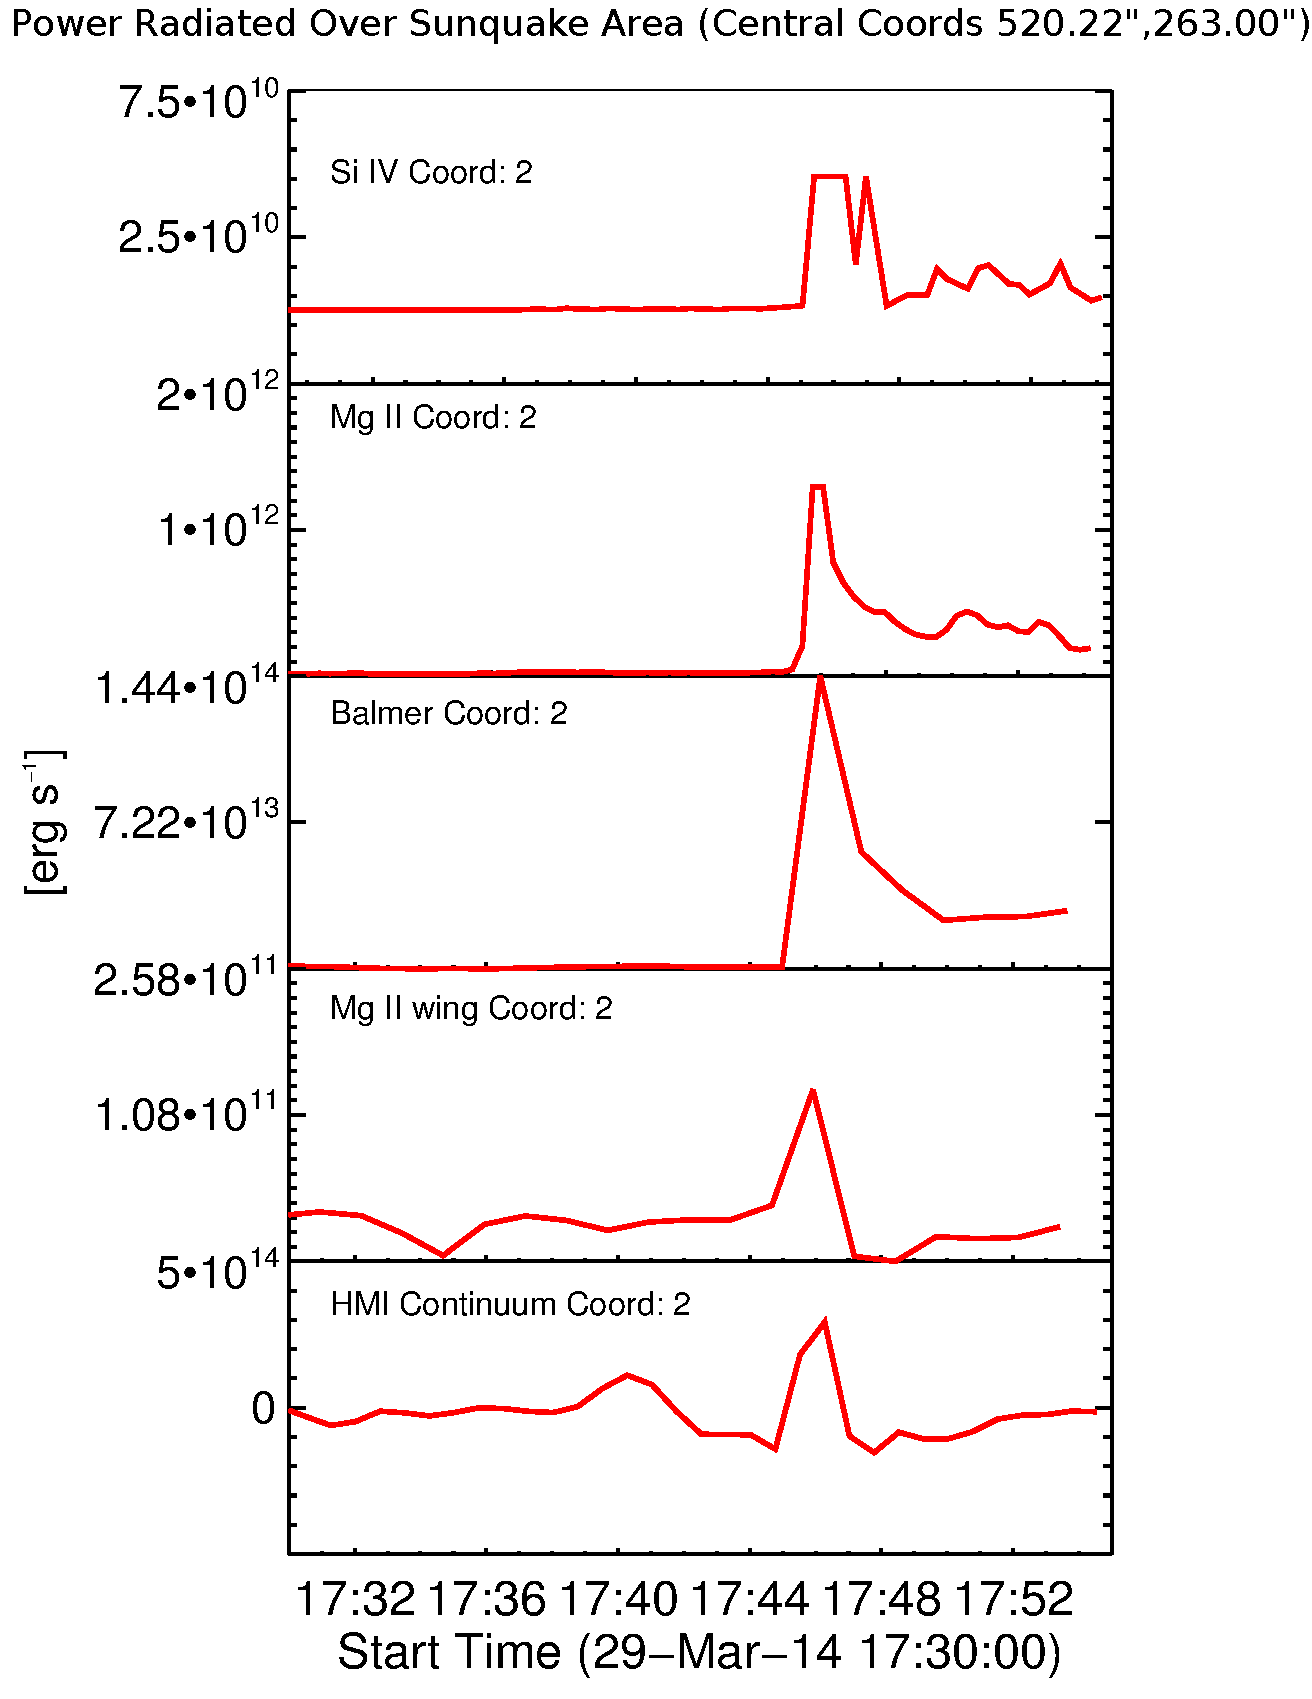
\includegraphics[width=0.6\textwidth]{29-Mar-14-Ribbon-Area-2-Sunquake-Area-Power-Ladder}
  \end{center}
  \caption{Shows radiative power from an area comparable to the sunquake impact, centered on region 2, which relates to heliocentric coordinates 520.2", 263.0". Each plot represents an independant data set, in order from top to bottom the sets are; IRIS SJ 1400 \AA\ (Si IV); IRIS SJ 2796 \AA\ (Mg II); IRIS SG  2825.7 to 2825.8 \AA\ (Balmer Continuum); IRIS SJ 2832 \AA\ (Mg II wing); SDO HMI continuum (HMI).}\label{plot2}
\end{figure}


\begin{figure}[H]
  \begin{center}
  \textbf{Quake Location Energy Over Time}\par\medskip
  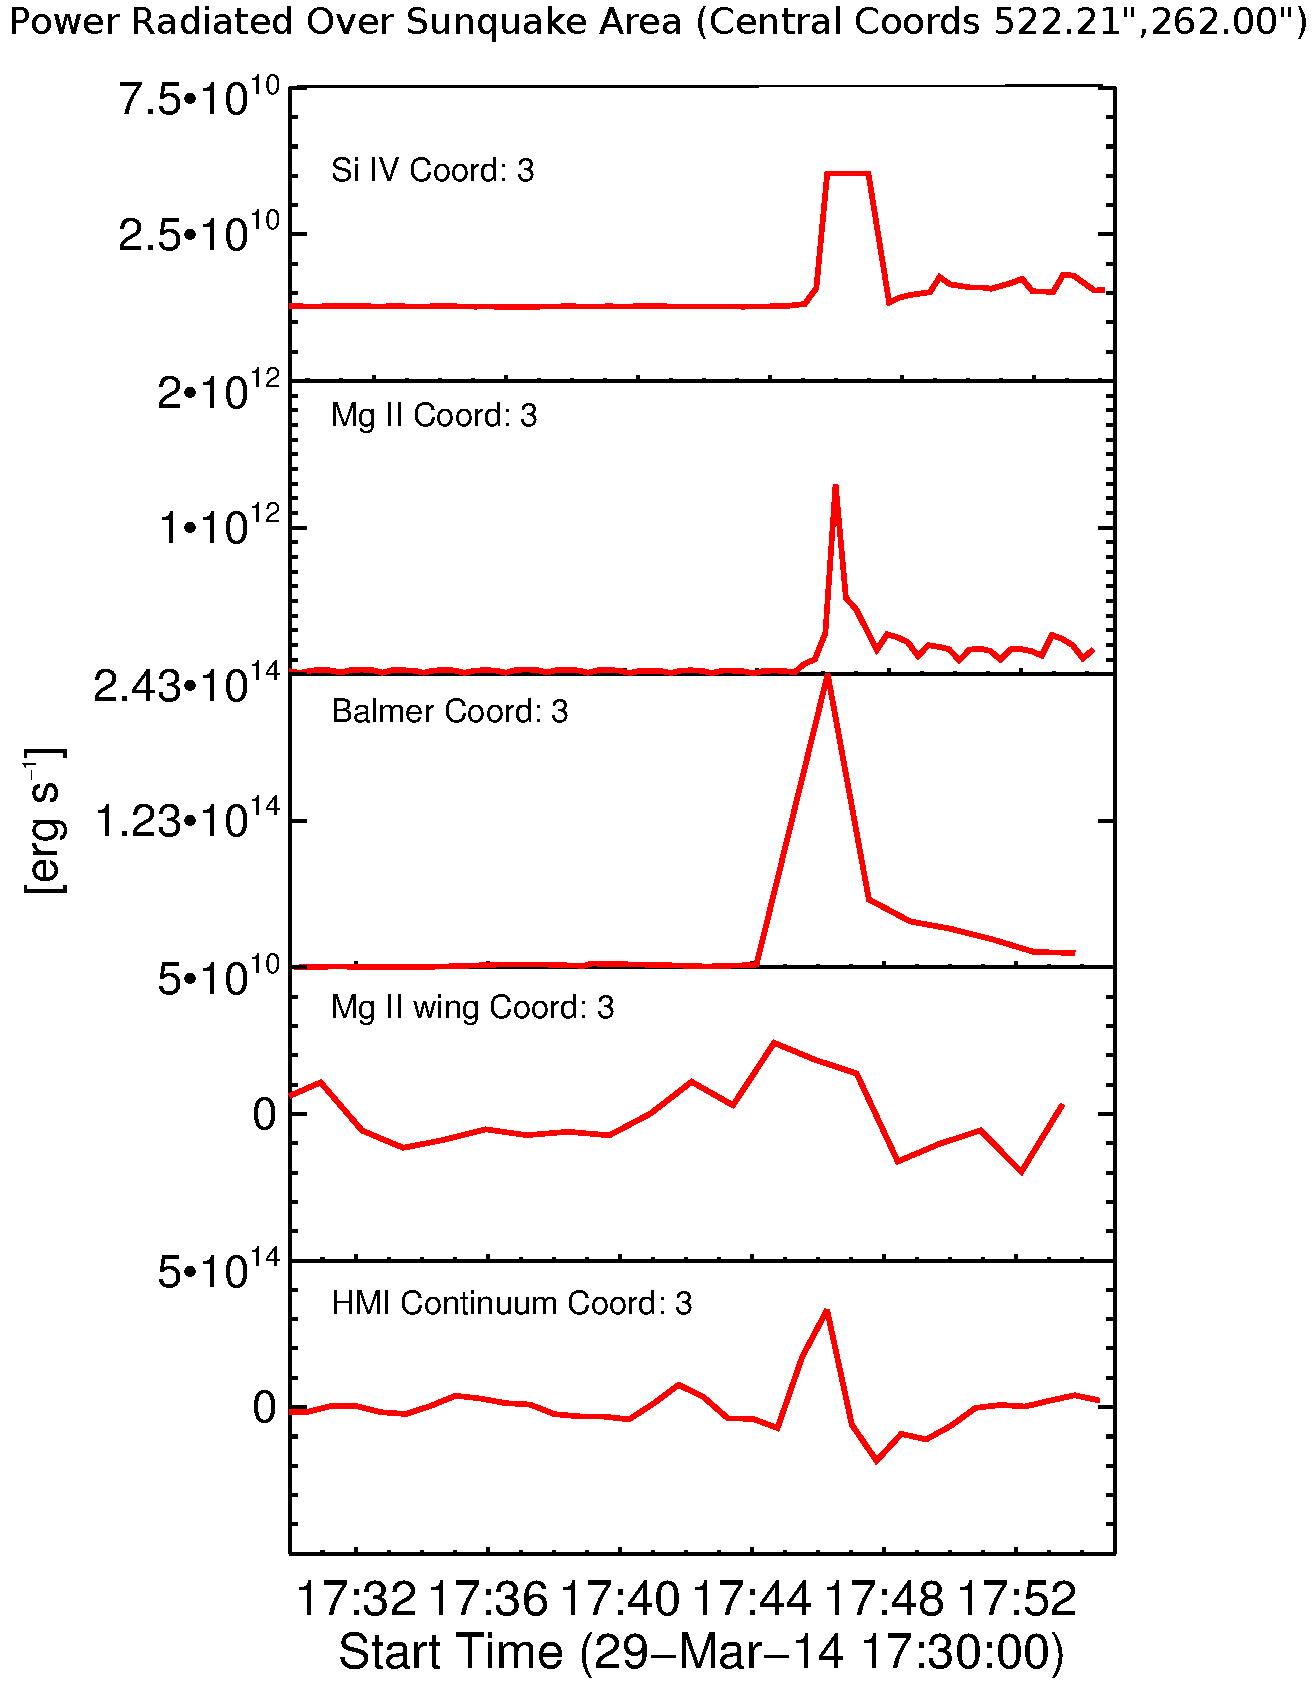
\includegraphics[width=0.6\textwidth]{29-Mar-14-Ribbon-Area-3-Sunquake-Area-Power-Ladder}
  \end{center}
  \caption{Shows radiative power from an area comparable to the sunquake impact, centered on region 3, which relates to heliocentric coordinates 522.2", 262.0". Each plot represents an independant data set, in order from top to bottom the sets are; IRIS SJ 1400 \AA\ (Si IV); IRIS SJ 2796 \AA\ (Mg II); IRIS SG  2825.7 to 2825.8 \AA\ (Balmer Continuum); IRIS SJ 2832 \AA\ (Mg II wing); SDO HMI continuum (HMI).}\label{plot3}
\end{figure}

\begin{figure}[H]
  \begin{center}
  \textbf{Quake Location Energy Over Time}\par\medskip
  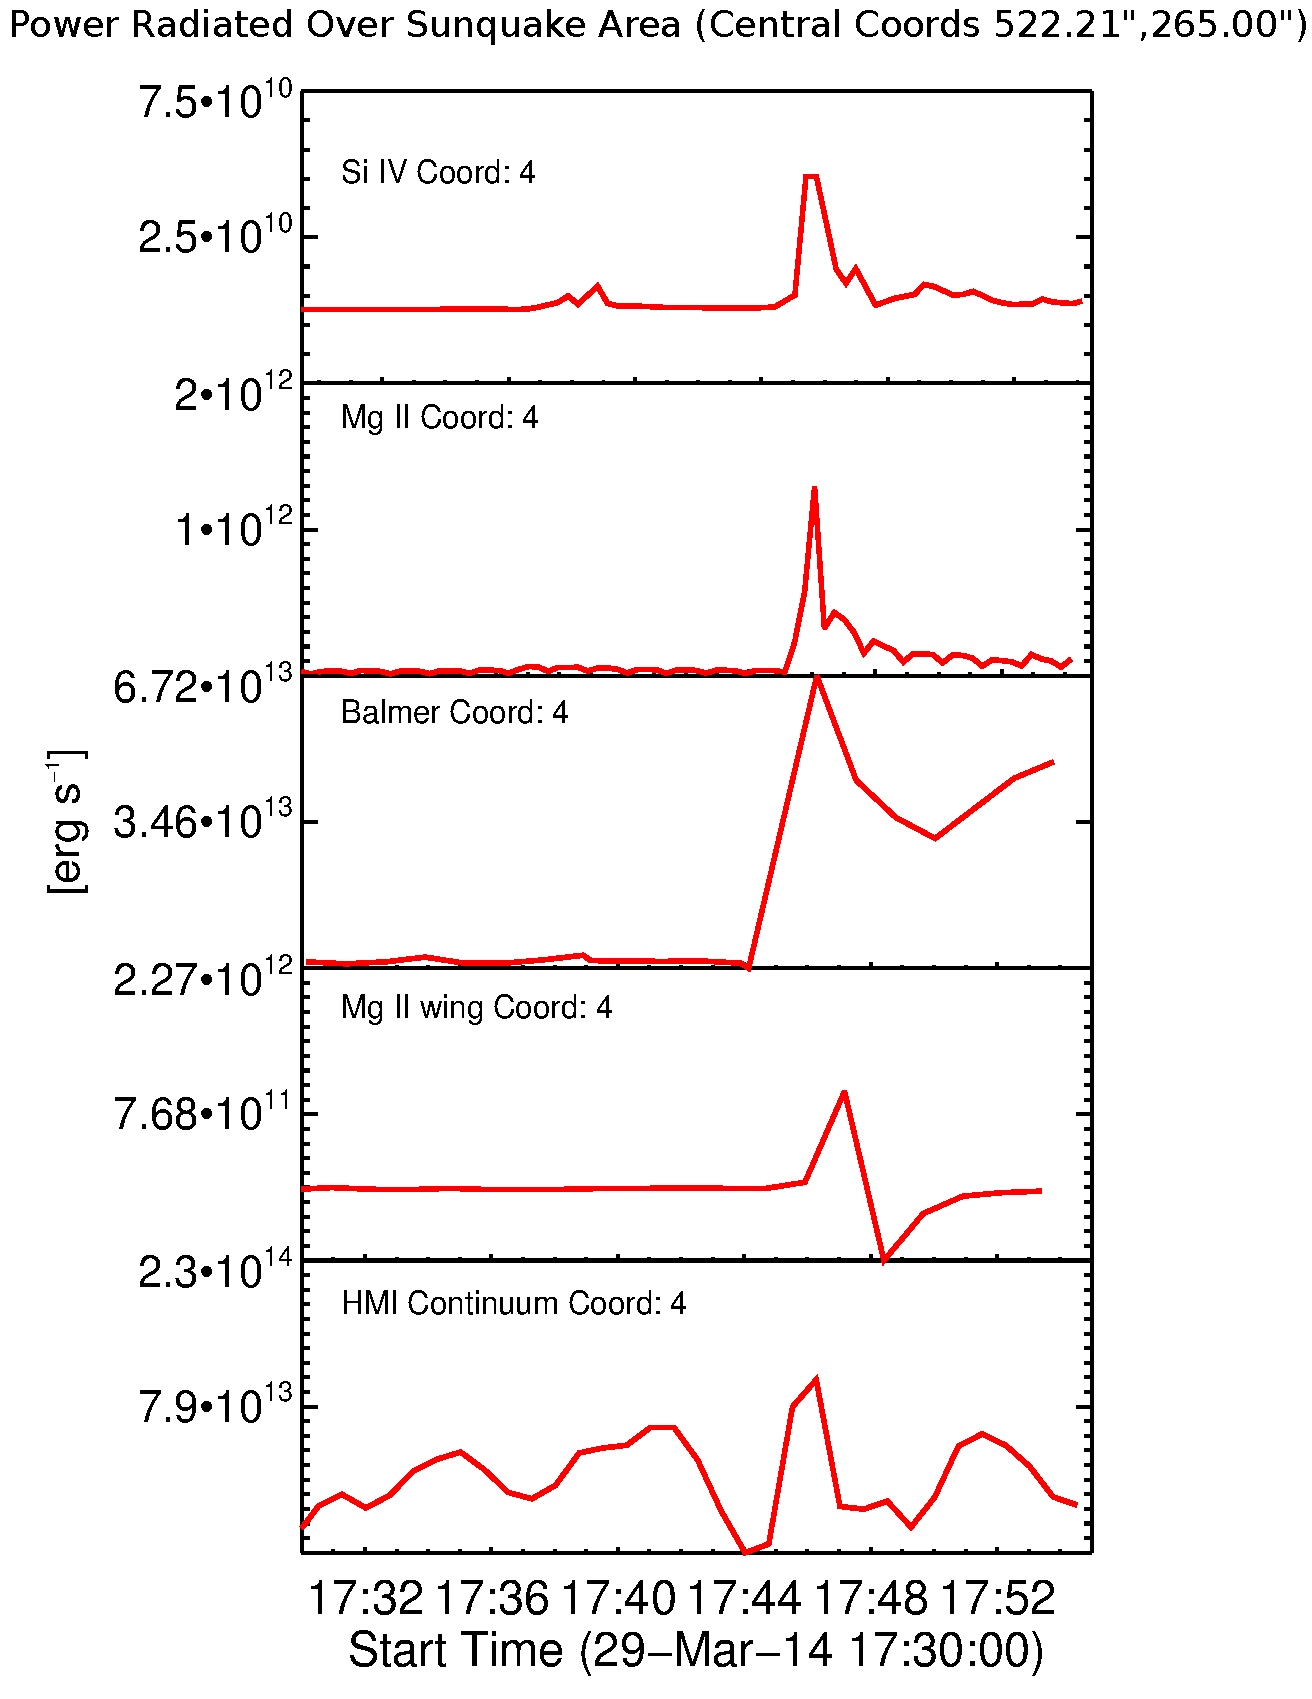
\includegraphics[width=0.6\textwidth]{29-Mar-14-Ribbon-Area-4-Sunquake-Area-Power-Ladder}
  \end{center}
  \caption{Shows radiative power from an area comparable to the sunquake impact, centered on region 4, which relates to heliocentric coordinates 522.2", 265.0". Each plot represents an independant data set, in order from top to bottom the sets are; IRIS SJ 1400 \AA\ (Si IV); IRIS SJ 2796 \AA\ (Mg II); IRIS SG  2825.7 to 2825.8 \AA\ (Balmer Continuum); IRIS SJ 2832 \AA\ (Mg II wing); SDO HMI continuum (HMI).}\label{plot4}
\end{figure}

\begin{figure}[H]
  \begin{center}
  \textbf{Quake Location Energy Over Time}\par\medskip
  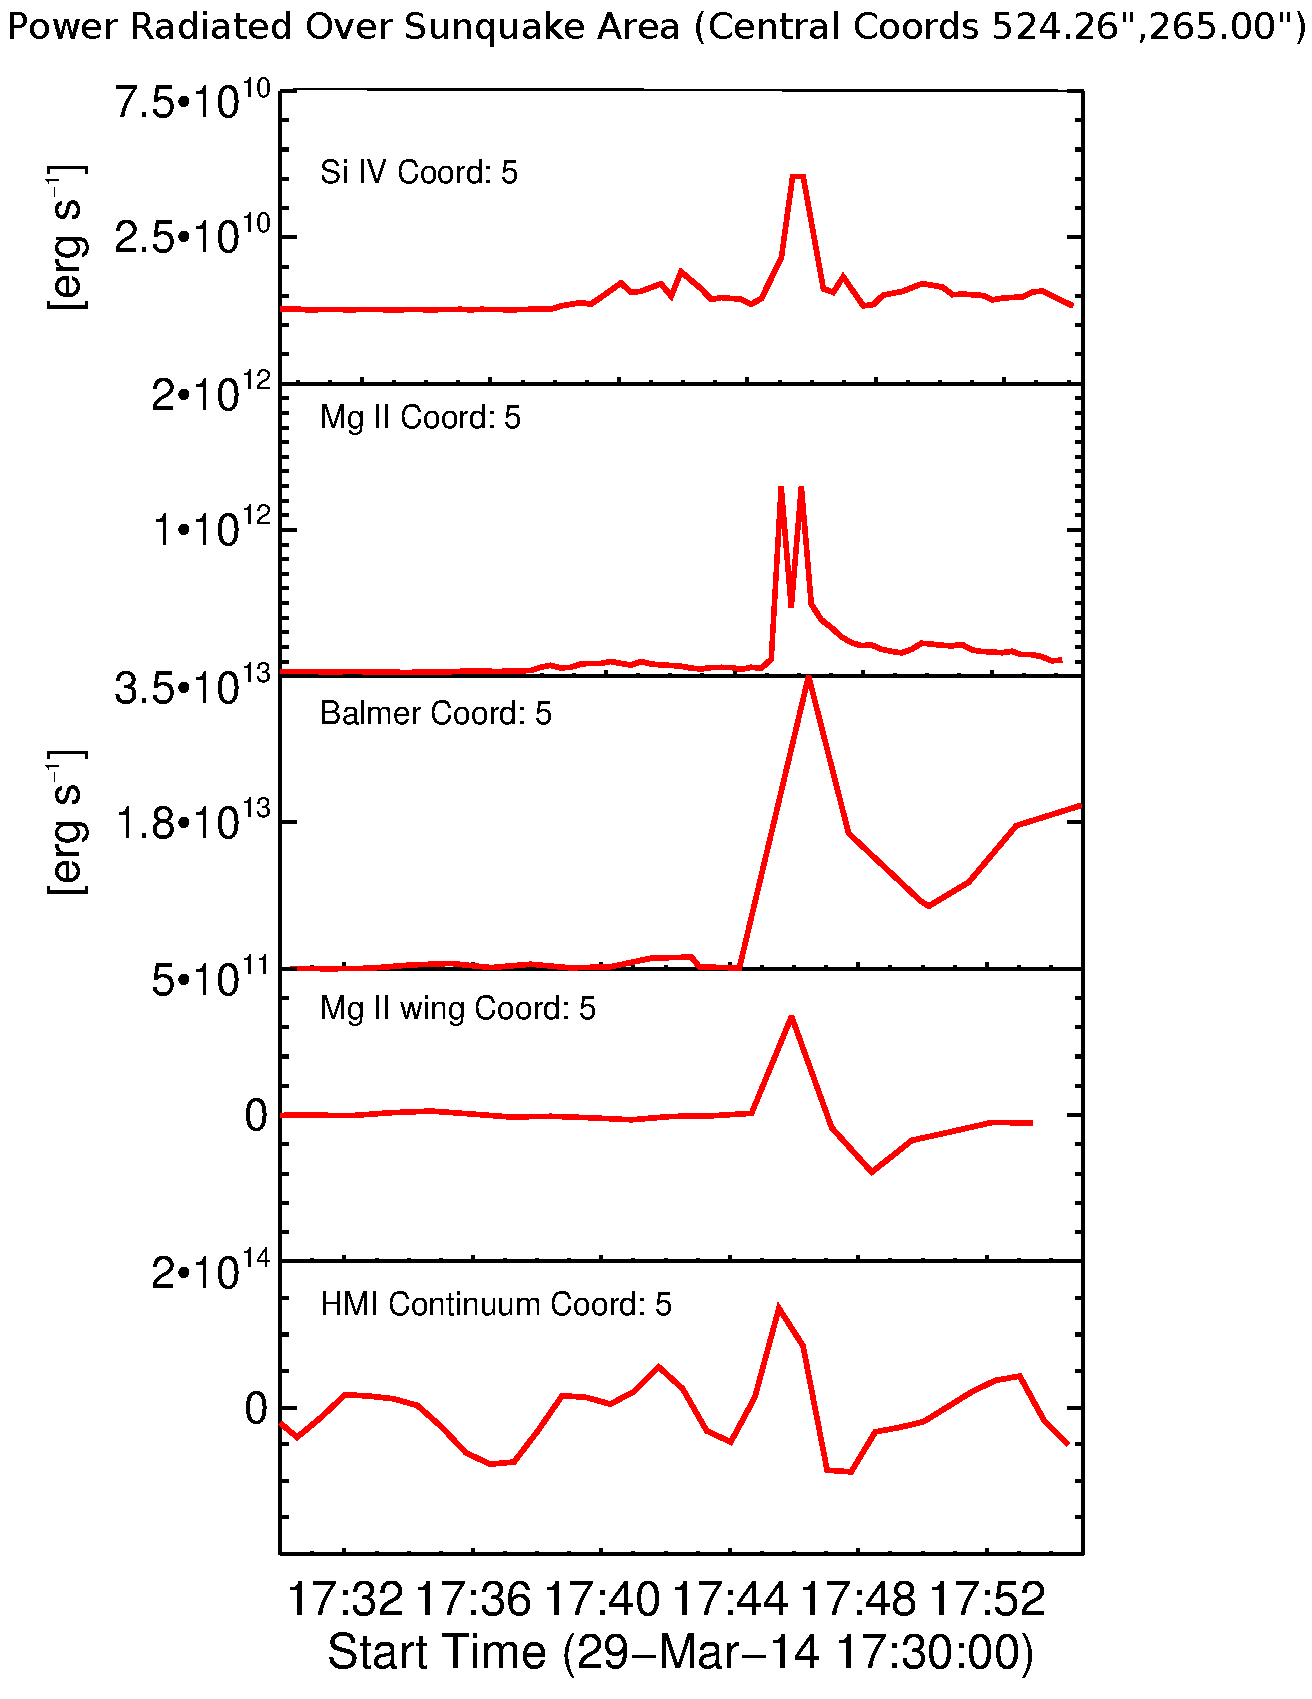
\includegraphics[width=0.6\textwidth]{29-Mar-14-Ribbon-Area-5-Sunquake-Area-Power-Ladder}
  \end{center}
  \caption{Shows radiative power from an area comparable to the sunquake impact, centered on region 5, which relates to heliocentric coordinates 524.3", 265.0". Each plot represents an independant data set, in order from top to bottom the sets are; IRIS SJ 1400 \AA\ (Si IV); IRIS SJ 2796 \AA\ (Mg II); IRIS SG  2825.7 to 2825.8 \AA\ (Balmer Continuum); IRIS SJ 2832 \AA\ (Mg II wing); SDO HMI continuum (HMI).}\label{plot5}
\end{figure}

\begin{figure}[H]
  \begin{center}
  \textbf{Quake Location Energy Over Time}\par\medskip
  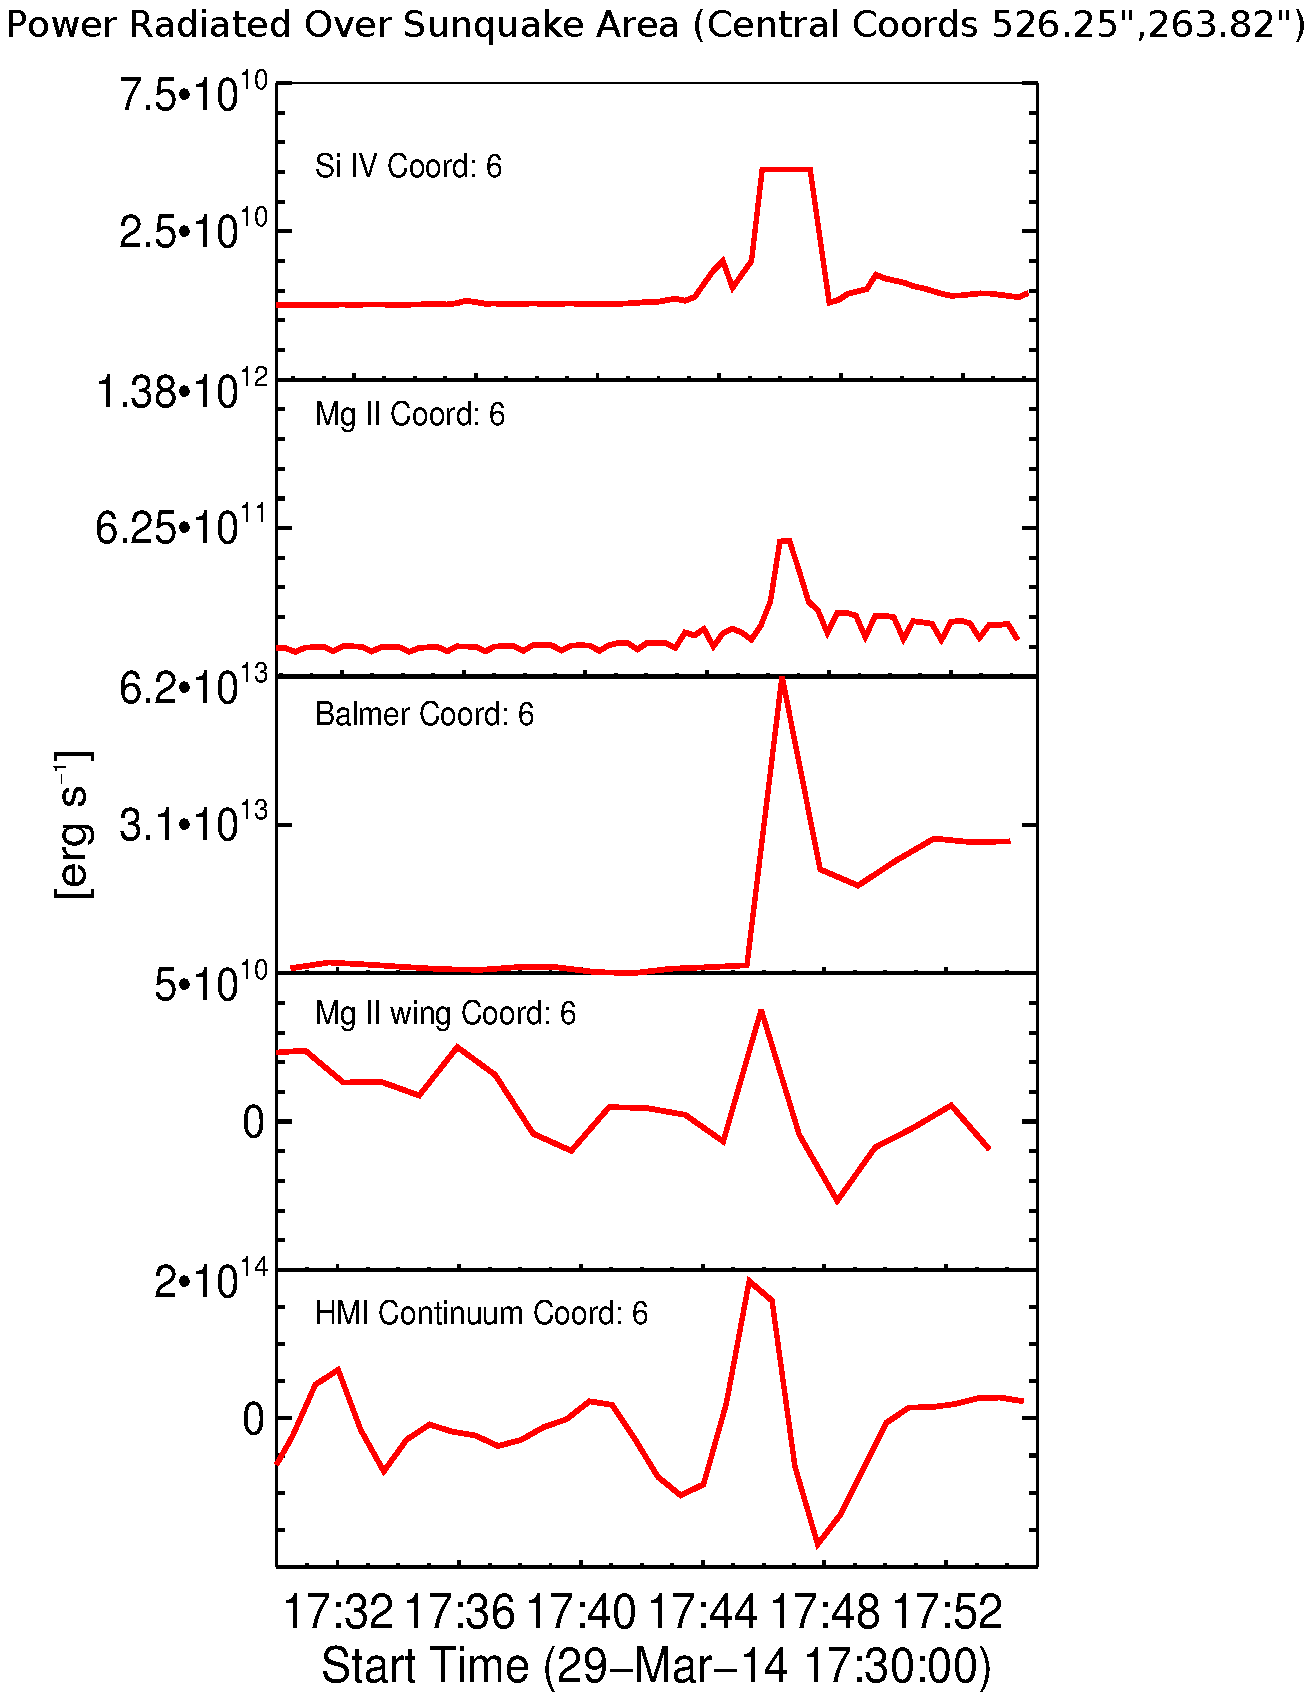
\includegraphics[width=0.6\textwidth]{29-Mar-14-Ribbon-Area-6-Sunquake-Area-Power-Ladder}
  \end{center}
  \caption{Shows radiative power from an area comparable to the sunquake impact, centered on region 6, which relates to heliocentric coordinates 526.3", 263.8". Each plot represents an independant data set, in order from top to bottom the sets are; IRIS SJ 1400 \AA\ (Si IV); IRIS SJ 2796 \AA\ (Mg II); IRIS SG  2825.7 to 2825.8 \AA\ (Balmer Continuum); IRIS SJ 2832 \AA\ (Mg II wing); SDO HMI continuum (HMI).}\label{plot6}
\end{figure}
